%%%%%%%%%%%%%%%%%%%%%%%%%%%%%%%%%%%%%%%%%%%%%%%%%%%%%%%%%%%%%%%%%%%
%                                                                 %
%  GEANT manual in LaTeX form                              %
%                                                                 %
%  Michel Goossens (for translation into LaTeX)                   %
%  Version 1.00                                                   %
%  Last Mod. Jan 24 1991  1300   MG + IB                          %
%                                                                 %
%%%%%%%%%%%%%%%%%%%%%%%%%%%%%%%%%%%%%%%%%%%%%%%%%%%%%%%%%%%%%%%%%%%
\Origin{L.Urb\'{a}n}
\Version{Geant 3.16}\Routid{PHYS431}
\Submitted{12.03.82}  \Revised{16.12.93}
\Makehead{Ionisation processes for heavy ions}

\section{Subroutines}

For a description of the subroutines used to calculate the energy
loss tables for protons, see {\tt [PHYS430]}.

\Shubr{GTHION}{}

\Rind{GTHION} transports heavy ions ($A,Z > 1$, particle
type 8). For the moment the
only discrete processes activated are $\delta$-ray and \v{C}erenkov
photon generation.

\section{Method}

The mean energy loss of the heavy ions can be expressed as:
\begin{equation}
\Delta E = Q^{2} S_{p} \left ( \frac{T}{A} \right ) \rho t
\end{equation}
where
\begin{DLtt}{MMMMMMMMM}
\item[$Q$] charge of the ion;
\item[$\displaystyle S_{p} \left ( \frac{T}{A} \right )$]
energy loss by the a proton with kinetic energy $T_{p} = T/A$;
\item[$T,A$] kinetic energy and mass number of the ion;
\item[$\rho$] density of the medium;
\item[$t$] step length
\end{DLtt}

This formula is used to calculate the ionisation loss for all the charged
hadrons.


In the case of ions, the charge of the ion makes the problem more difficult.
Electron-exchange processes with the atoms change the
charge as the ion traverses the medium. The main features of this 
process can be summarised as follows:
\begin{itemize}
\item $Q$ loses the dependence on the initial ion charge after a
very short initial step, usually $\ll 1\mu$ for condensed media;
\item $Q$ does depend on the velocity of the ion;
\item even in the case of constant velocity, $Q$ fluctuates around
a mean value;
\item $Q$ features a small dependence on the medium, especially for
small values of $T$.
\end{itemize}
\begin{table}
\begin{centering}
\begin{tabular}{|c|c|c|}
\hline
T/A & He ions & Pb ions \\
MeV & error (\%) & error (\%) \\
\hline
10 & 3 &  1 \\
5 & 4 & 3 \\
3 & 10 & 4 \\
\hline
\end{tabular}
\caption{Comparison of the measured and calculated $\Delta$E for 10 MeV/A
ions in Pb}
\end{centering}
\label{tb:phys431-1}
\end{table}

If we want to calculate the energy loss of the ion, we need a good
parametrisation for the quantity $Q=Q_{eff}$. We give here a 
relatively simple parametrisation~\cite{bib-ANZI,bib-ANZ1}:
\begin{eqnarray}
\label{eq:phys431-2}
Q_{eff} & = & Z_{I} \left [ 1- \left ( 1.034 - 0.1777 e^{-0.08114\;Z_{I}}
\right ) e^{-v} \right ] \\
v & = & 121.4139 \frac{\beta}{Z_{I}^{2/3}} + 0.0378
\sin \left ( 190.7165 \frac{\beta}{Z_{I}^{2/3}} \right ) \nonumber
\end{eqnarray}
where $\beta$ is the velocity and $Z_{I}$ the atomic number of the ion
(i.e. the charge of the bare nucleus).

\begin{table}
\begin{centering}
\begin{tabular}{|r|rr|rr|r|r|rr|rr|r|r|}
\hline
\multicolumn{1}{|c|}{T (MeV)} & \multicolumn{6}{c|}{417 $\mu$g cm$^{-2}$}
& \multicolumn{6}{c|}{110 $\mu$g cm$^{-2}$} \\[0.1cm]
& \multicolumn{4}{c|}{MC (keV)} & \multicolumn{2}{c|}{data (keV)} &
\multicolumn{4}{c|}{MC (keV)} & \multicolumn{2}{c|}{data (keV)} \\
& $\Delta$E & dif & FWHM & dif & $\Delta$E & FWHM & 
$\Delta$E & dif & FWHM & dif & $\Delta$E & FWHM \\
\hline
4.88  & &  & & & & & 785 & 8 & 59 & -23 & 725 & 77 \\
9.85 & 3600 & 14 & 138 & -33 & 3150 & 206 & 816 & 8 & 67 &  -26 & 756 & 91 \\
19.79 & 3090 & 3 & 142 & -35 & 2990 & 218 & 719 & 3 & 70 & -32 & 699 & 103 \\
29.27 & 2660 & 1 & 141 & -31 & 2630 & 204 & & & & & & \\
29.75 & & & & & & & 620 & 4 & 69 & -26 & 598 & 93 \\
39.70 & 2320 & 1 & 138 & -28 & 2300 & 191 & 550 & 4 & 68 & -24 & 528 & 90 \\
\hline
\end{tabular}
\caption{Comparison of the measured and calculated $\Delta$E and FWHM
for O ions in Al; errors are in percent.}
\end{centering}
\label{tb:phys431-2}
\end{table}

It can be seen that (\ref{eq:phys431-2}) neglects the (small) medium
dependence of $Q_{eff}$. For very high energies ($\beta \rightarrow 1$)
$Q_{eff} \rightarrow Z_{I}$. For very low energies ($T/A \sim$ few keV)
the formula breaks down. $Q_{eff}$ can even become negative for $T/A <
20$ keV and $Z_{I} > 20$. However this is not a serious source of
error when calculating $\Delta E$, since in this case the range of
the ion is very small, and it can almost be said that it stops
{\it immediately}.

The calculation of the energy loss straggling (fluctuations) differs
from that of {\it normal} charged hadrons. For the charged hadrons
the fluctuations come from the statistical nature of the 
projectile-atom interactions; for the ions there is another process which
broadens the energy loss distribution: the fluctuation of the charge.
For heavier ions this process dominates the energy loss straggling
for $T/A \leq 10$ MeV.

\begin{figure}[hbt]
     \centering
     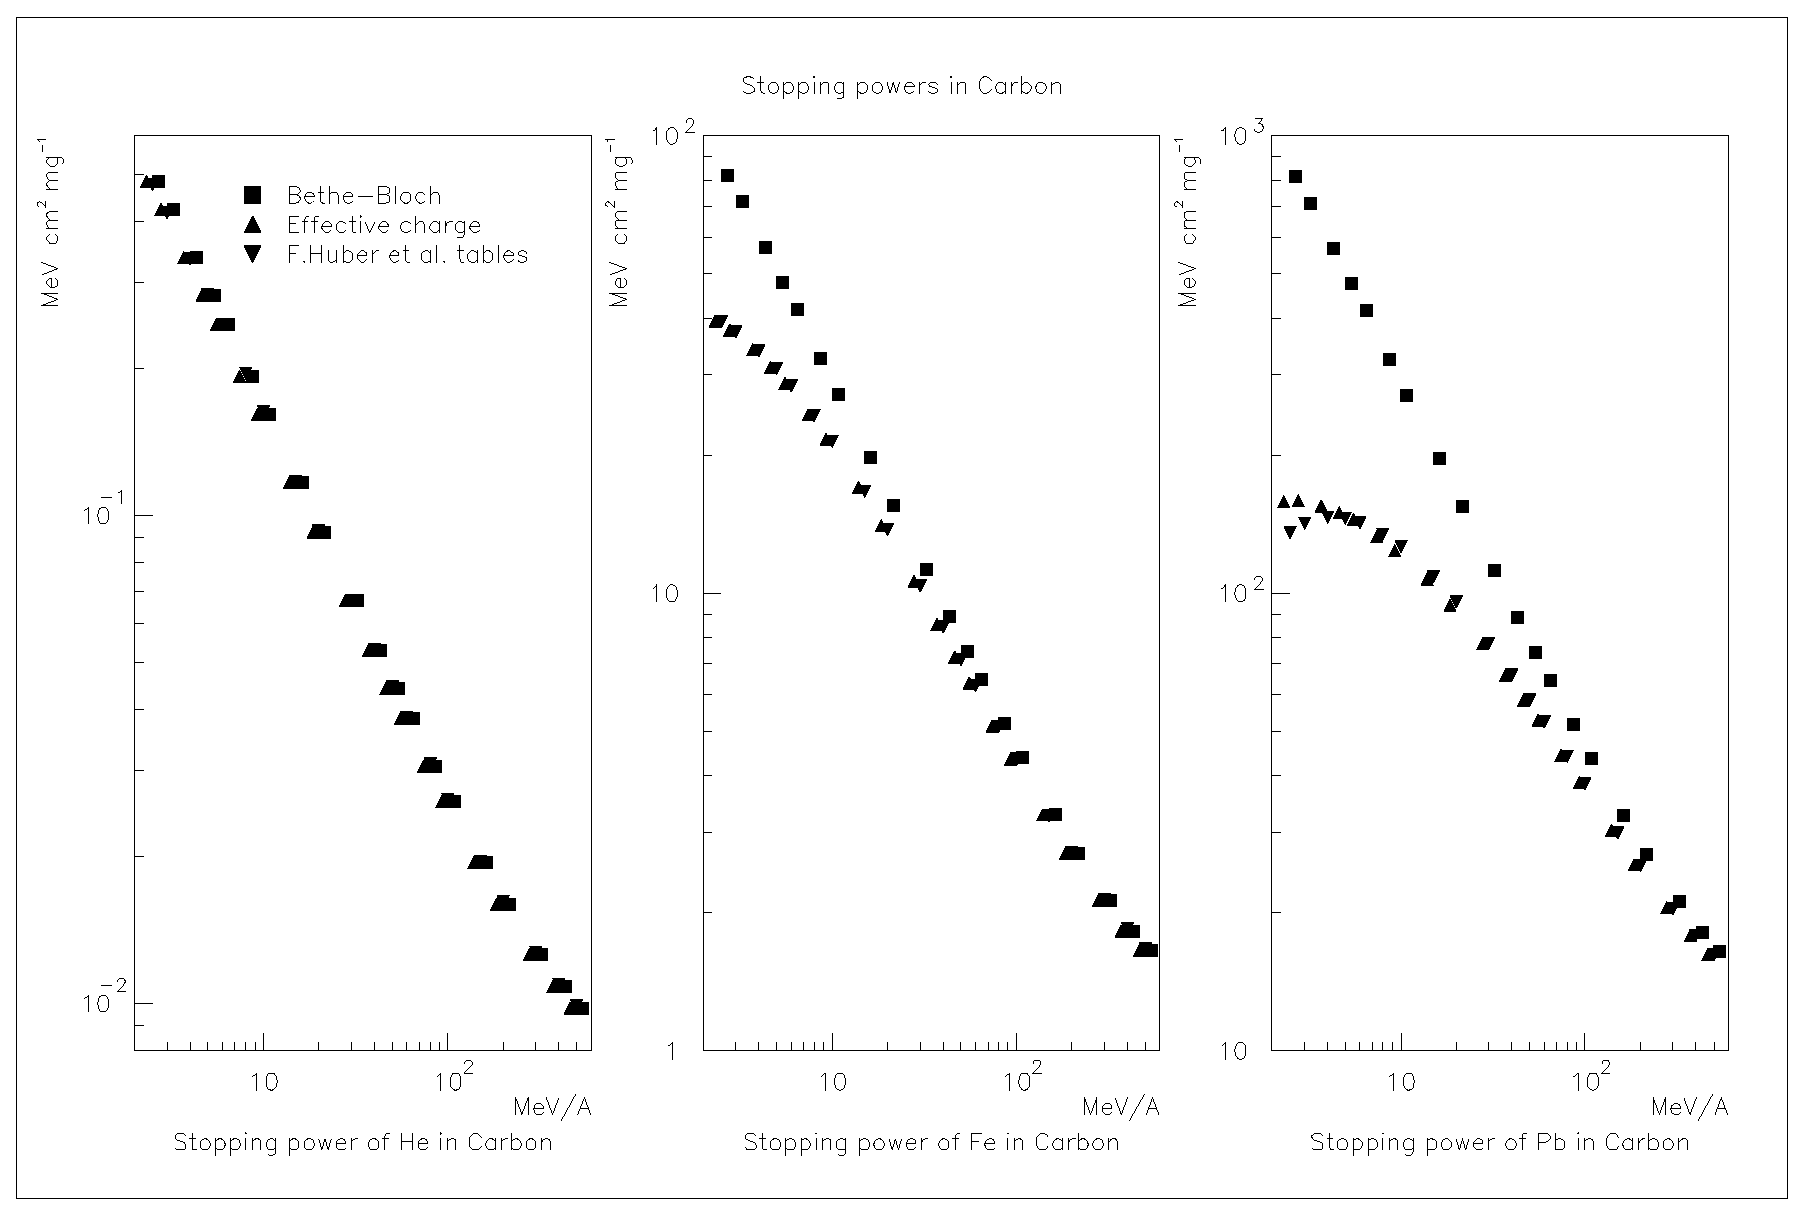
\epsfig{file=eps/phys431-1.eps,width=14cm}
     \caption{Stopping powers in Carbon}
     \label{fg:phys431-1}
\end{figure}

The heavy ions are in the {\it Gaussian regime} (see {\tt [PHYS332]})
of the collisional fluctuations even in the case of very thin absorbers.
If $T/A$ is not too high, the $\sigma^{2}$ of the distribution:
\begin{equation}
\label{eq:phys431-3}
\sigma^{2}_{coll} = D \frac{Q_{eff}^{2} Z}{A} \rho \; t \; m
\left [ 1 + \frac{T_{A}}{M_{u}} + \frac{1}{2} \left ( \frac{T_{A}}{M_{u}}
\right ) ^{2} \right ]
\end{equation}
where
\begin{DLtt}{MMMMMMMM}
\item[$D$] $\displaystyle 0.307 \frac{\mbox{MeV cm$^{2}$}}{\mbox{g}}$;
\item[$T_{A}$] $\displaystyle \frac{T}{A}$;
\item[$M_{u}$] atomic mass unit;
\item[$Z$] atomic number of the medium;
\item[$A$] mass number of the medium.
\end{DLtt}

\begin{table}
\begin{centering}
\begin{tabular}{|r|rr|r|rr|r|rr|r|}
\hline
& \multicolumn{9}{c|}{Pb ions in gas (energies in MeV)} \\
& \multicolumn{3}{c|}{N$_{2}$} & 
\multicolumn{3}{c|}{Ar} & 
\multicolumn{3}{c|}{Xe} \\
& \multicolumn{2}{c}{MonteCarlo} & \multicolumn{1}{c|}{data} &
\multicolumn{2}{c}{MonteCarlo} & \multicolumn{1}{c|}{data} &
\multicolumn{2}{c}{MonteCarlo} & \multicolumn{1}{c|}{data} \\
t (cm) & 
$\Delta$E & FWHM & FWHM & $\Delta$E & FWHM & FWHM & $\Delta$E & FWHM & FWHM \\
\hline
0.2 & 25.9 & 1.15 & 1.1 & 25.4 & 1.30 & 1.4 & 51.1 & 2.26 & 2.5 \\
0.4 & 53.6 & 1.62 & 1.5 & 52.4 & 1.84 & 1.9 & 107.0 & 3.22 & 3.3 \\
0.8 & 112.0 & 2.25 & 2.0 & 111.0 & 2.59 & 2.6 & 236.0 & 4.51 &  \\
1.2 & 162.0 & 2.37 & 2.0 & 168.0 & 2.95 & 2.8 & & & \\
\hline
\end{tabular}
\caption{Comparison of the measured and calculated and FWHM
for 1.4 MeV/A Pb ions in gas.}
\end{centering}
\label{tb:phys431-3}
\end{table}

Analysing the experimental straggling data it is possible to find that
the electron-exchange charge fluctuations can be described by a Gaussian
with width:
\begin{equation}
\label{eq:phys431-4}
\sigma^{2}_{ch} = D \frac{Q_{eff}^{2} Z}{A} \rho \; t \; m \frac{C}{2}
\left ( 1 - \frac{Q_{eff}}{Z_{I}} \right )
\end{equation}
where the parameter $C \sim 2.5$ has been derived
from the experimental straggling data.

If $Q_{eff} \rightarrow Z_{I}$, which is the case for high energy
heavy ions and for few MeV/A He ions, then $\sigma^{2}_{ch} \rightarrow 0$.


Comparing equations (\ref{eq:phys431-3}) and (\ref{eq:phys431-4}) it can be 
seen that for heavy ions and for $T/A \ll M_{u}$ $\sigma^{2}_{ch}
> \sigma^{2}_{coll}$. The total energy loss fluctuation can be
described by a Gaussian distribution with:
\begin{equation}
\sigma^{2} = \sigma^{2}_{ch} + \sigma^{2}_{coll}
\end{equation}

The mean energy loss and energy loss fluctuation calculation is performed
in the routine \Rind{GTHION}, making use of the proton energy loss tables.

{\bf Note:} The Gaussian fluctuation gives too broad a distribution for
high energy in the case of thin absorbers. A correction has been introduced
in \Rind{GTHION} which cures this discrepancy. In the absence of high
energy straggling data for ions, the correction has been tuned using 
high energy $\pi$ energy loss data, where the $\pi$ has been tracked
by \Rind{GTHION}.

\section{Comparison with data}

\subsection{Mean energy loss and range}

A test has been made against the distributions reported in~\cite{bib-HEIN}
for He ions at 1 and 10 MeV/A and for O and Pb ions at 1, 10 and
100 MeV/A in carbon and the results were found
to be correct within $5\%$ both for the energy loss and the range.

\begin{figure}[hbt]
     \centering
     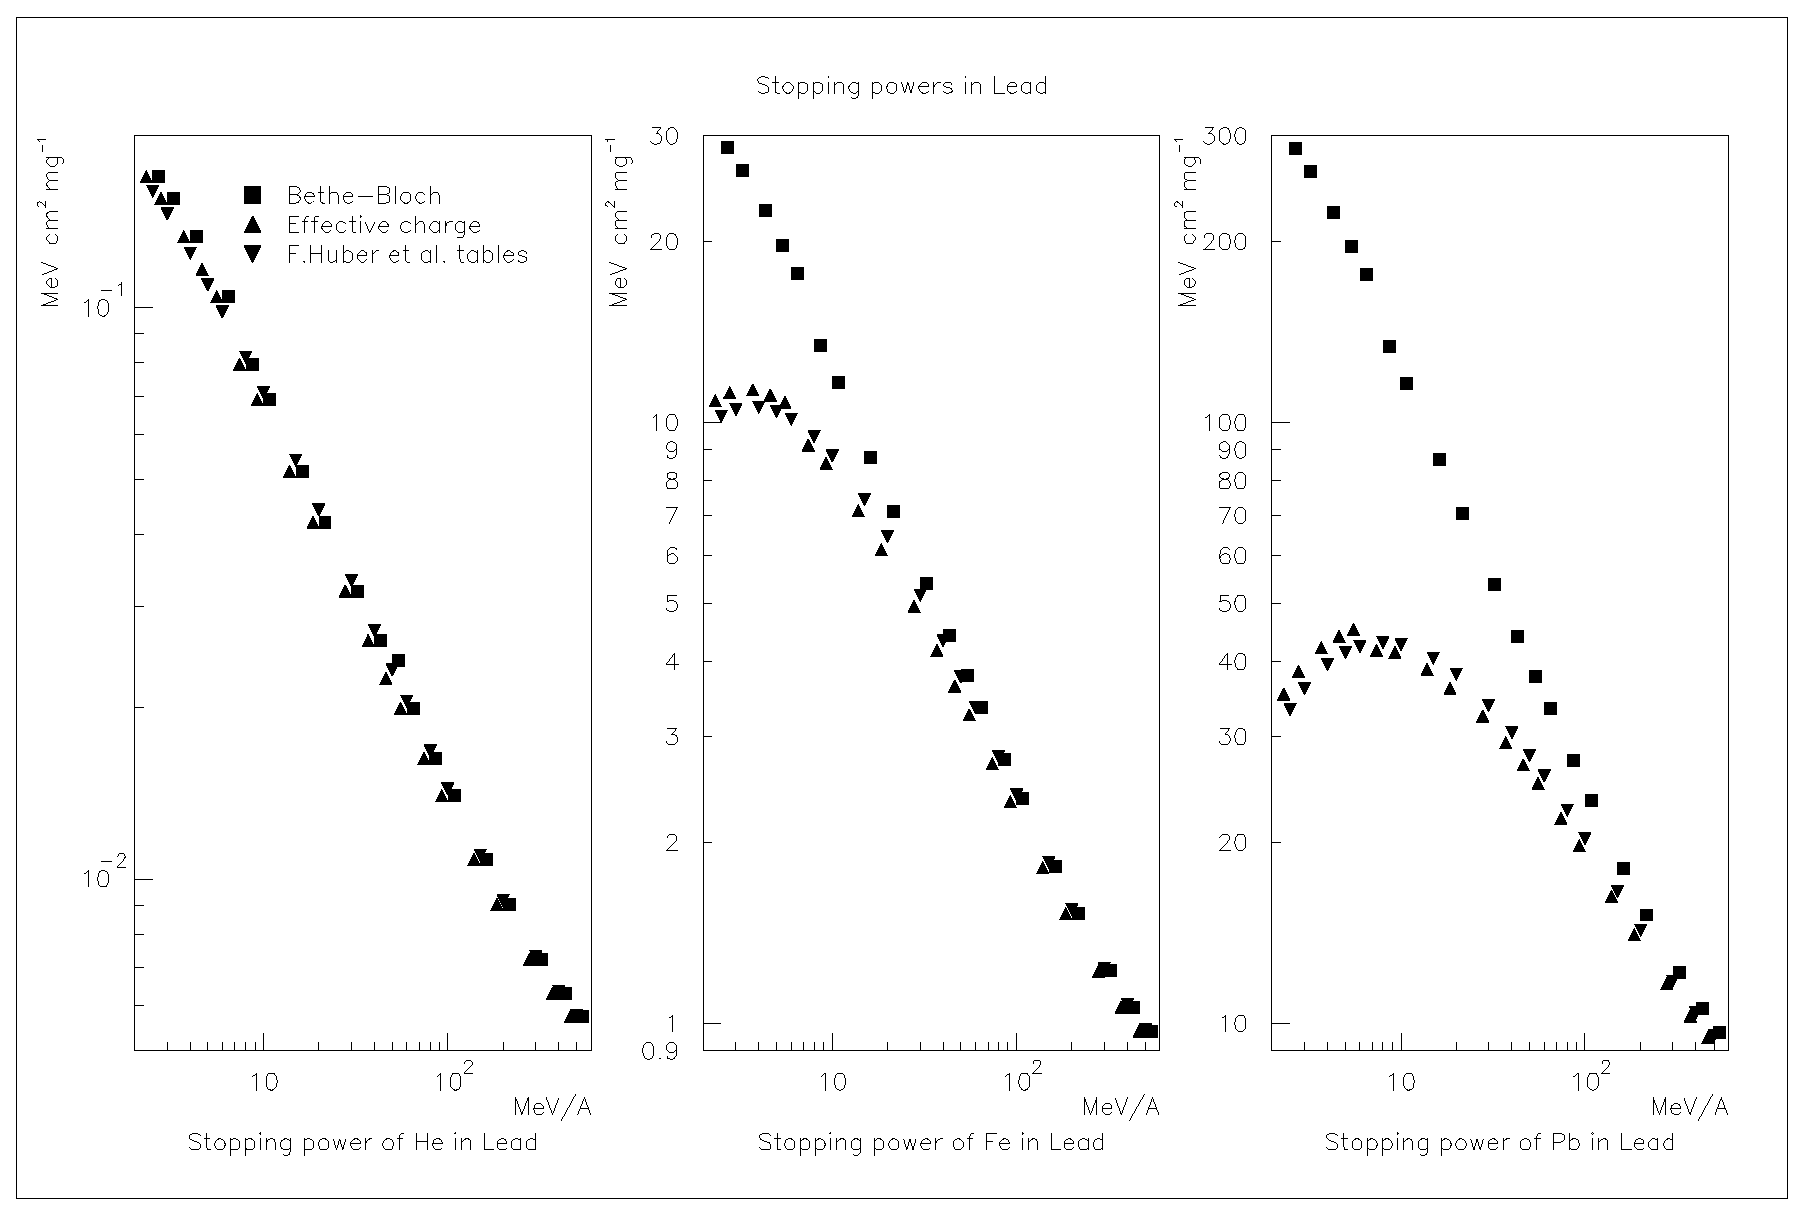
\epsfig{file=eps/phys431-2.eps,width=14cm}
     \caption{Stopping powers in Lead}
     \label{fg:phys431-2}
\end{figure}

Another comparison has been made with the tables of~\cite{bib-HUBE} 
for 10 MeV/A ions in lead, with
the results shown in table~\ref{tb:phys431-1}.
Another comparison with the same tables is shown in Figs.~\ref{fg:phys431-1}
and \ref{fg:phys431-2}.

A comparison with the tables in~\cite{bib-ANZI,bib-ANZ1} for T/A $<$ 1 MeV/A
gives  an error on $(dE/dx) \leq 10-20\%$.

\begin{table}
\begin{centering}
\begin{tabular}{|r|rr|r|}
\hline
\multicolumn{4}{|c|}{He ions in Ar (energies in keV)} \\
& \multicolumn{2}{c}{MonteCarlo} & \multicolumn{1}{c|}{data} \\
t (cm) & 
$\Delta$E & FWHM & FWHM \\
\hline
0.5 & 444 & 38 & $\sim$40 \\
1.0 & 913 & 53 & $\sim$60 \\
2.0 & 1940 & 78 & $\sim$80 \\
\hline
\end{tabular}
\caption{Comparison of the measured and calculated and FWHM
for 1.4 MeV/A He ions in gas.}
\end{centering}
\label{tb:phys431-4}
\end{table}

\subsection{Comparison of FWHM}

A comparison has been made with 
low energy data ($0.3 \leq T/A \leq 2.5$ MeV/A) in very
thin absorbers (1,7 $\mu$m, 0.4 $\mu$m). Data are taken from
the tables in~\cite{bib-TSCH} for
energy loss of O ions in Al, and the
results are reported in table~\ref{tb:phys431-2}. The quoted experimental 
error for these data is $1\%$ statistical + $5\%$ systematic for 
417 $\mu$g cm$^{-2}$ data and $2\%$ statistical + $10\%$ systematic for
110 $\mu$g cm$^{-2}$ data. 

Plots of energy deposition distributions of 1.4 MeV/A lead and helium
ions in gases can be found in~\cite{bib-GEIS}. 
From these we have measured the FWHM and compared them with the ones given
by the MonteCarlo. The results can be seen in table~\ref{tb:phys431-3}
and ~\ref{tb:phys431-4}. It
should be noted that the absorber thickness of, for example, Ar compares
with that of the preceding case (0.2 cm Ar = 356 $\mu$g cm$^{-2}$ and
1.2 cm Ar = 2136 $\mu$g cm$^{-2}$).


Similar comparison has been made for C ions of energies 17.1 and 39.4 MeV in 
isobuthane~\cite{bib-SCHM} and the agreement between data and {\tt GEANT}
for FWHM is within 30\%.
